% Generated by simulate-hypergeometric.py. Do not edit numerical data by hand.
% Fragment only: requires amsmath, xcolor, and PGFPlots compat=1.18.
% No groupplots library, external images, data files, or shell escape required.
% Each panel is unbreakable; page breaks are allowed between panels.
\begingroup
\noindent\textbf{A fixed sample from a growing population.}
Keep the sample size $n=10$ and success fraction $p=K/N=1/2$ fixed.
Increase the population through $N=12,40,400$, with $K=N/2$ successes.
Sampling is without replacement within each sample; the population is reset
before the next Monte Carlo repetition.

\smallskip
\noindent Blue bars are the \textbf{exact hypergeometric probabilities}.
Orange open diamonds are the \textbf{exact $\operatorname{Bin}(10,1/2)$ probabilities}.
Black crosses are \textbf{Monte Carlo relative frequencies} from $100{,}000$
repetitions per panel. Marks refer only to integer counts, not a density.
All panels have the same axes, show every count $k=0,\ldots,10$, and omit no mass.

\par\medskip
\noindent\begin{minipage}{\linewidth}
\centering
{\small\bfseries Population $N=12$, with $K=6$ successes; sample $n=10$}\par
{\small Sample fraction $n/N=83.33\%$; exact support $\{4,5,6\}$; exact variance $0.454545$}\par
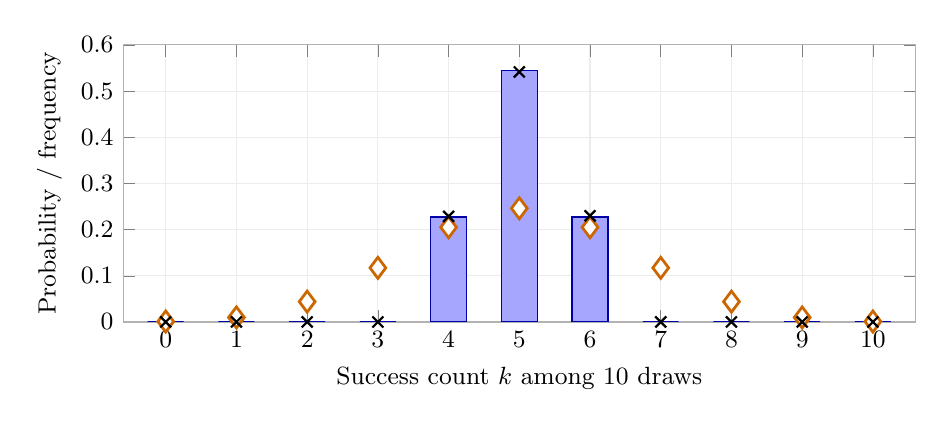
\begin{tikzpicture}
\begin{axis}[
  width=0.96\linewidth,height=5.1cm,
  xmin=-0.6,xmax=10.6,ymin=0,ymax=0.60,
  xtick={0,1,...,10},ytick={0,0.1,...,0.6},
  xlabel={Success count $k$ among $10$ draws},ylabel={Probability / frequency},
  tick label style={font=\small},label style={font=\small},
  scaled y ticks=false,grid=major,grid style={gray!15},
  axis line style={gray!60}]
\addplot[ybar,bar shift=0pt,bar width=13pt,
  fill=blue!35,draw=blue!65!black] coordinates {
  (0,0)
  (1,0)
  (2,0)
  (3,0)
  (4,0.22727272727273)
  (5,0.54545454545455)
  (6,0.22727272727273)
  (7,0)
  (8,0)
  (9,0)
  (10,0)
};
\addplot[only marks,mark=diamond*,mark size=3.8pt,
  color=orange!80!black,mark options={fill=white,line width=1pt}] coordinates {
  (0,0.0009765625)
  (1,0.009765625)
  (2,0.0439453125)
  (3,0.1171875)
  (4,0.205078125)
  (5,0.24609375)
  (6,0.205078125)
  (7,0.1171875)
  (8,0.0439453125)
  (9,0.009765625)
  (10,0.0009765625)
};
\addplot[only marks,mark=x,mark size=2.8pt,
  color=black,mark options={line width=0.8pt}] coordinates {
  (0,0)
  (1,0)
  (2,0)
  (3,0)
  (4,0.2286)
  (5,0.54144)
  (6,0.22996)
  (7,0)
  (8,0)
  (9,0)
  (10,0)
};
\end{axis}
\end{tikzpicture}
\end{minipage}

\par\medskip
\noindent\begin{minipage}{\linewidth}
\centering
{\small\bfseries Population $N=40$, with $K=20$ successes; sample $n=10$}\par
{\small Sample fraction $n/N=25.00\%$; exact support $\{0,1,\ldots,10\}$; exact variance $1.923077$}\par
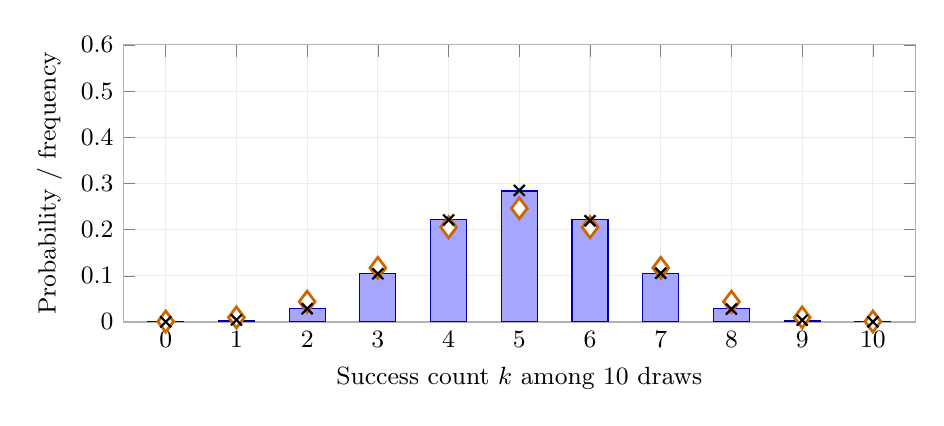
\begin{tikzpicture}
\begin{axis}[
  width=0.96\linewidth,height=5.1cm,
  xmin=-0.6,xmax=10.6,ymin=0,ymax=0.60,
  xtick={0,1,...,10},ytick={0,0.1,...,0.6},
  xlabel={Success count $k$ among $10$ draws},ylabel={Probability / frequency},
  tick label style={font=\small},label style={font=\small},
  scaled y ticks=false,grid=major,grid style={gray!15},
  axis line style={gray!60}]
\addplot[ybar,bar shift=0pt,bar width=13pt,
  fill=blue!35,draw=blue!65!black] coordinates {
  (0,0.00021795989537925)
  (1,0.0039629071887136)
  (2,0.028235713719585)
  (3,0.10425494296462)
  (4,0.22154175379982)
  (5,0.28357344486377)
  (6,0.22154175379982)
  (7,0.10425494296462)
  (8,0.028235713719585)
  (9,0.0039629071887136)
  (10,0.00021795989537925)
};
\addplot[only marks,mark=diamond*,mark size=3.8pt,
  color=orange!80!black,mark options={fill=white,line width=1pt}] coordinates {
  (0,0.0009765625)
  (1,0.009765625)
  (2,0.0439453125)
  (3,0.1171875)
  (4,0.205078125)
  (5,0.24609375)
  (6,0.205078125)
  (7,0.1171875)
  (8,0.0439453125)
  (9,0.009765625)
  (10,0.0009765625)
};
\addplot[only marks,mark=x,mark size=2.8pt,
  color=black,mark options={line width=0.8pt}] coordinates {
  (0,0.00022)
  (1,0.0043)
  (2,0.02866)
  (3,0.10432)
  (4,0.22084)
  (5,0.28487)
  (6,0.21916)
  (7,0.10557)
  (8,0.02791)
  (9,0.00384)
  (10,0.00031)
};
\end{axis}
\end{tikzpicture}
\end{minipage}

\par\medskip
\noindent\begin{minipage}{\linewidth}
\centering
{\small\bfseries Population $N=400$, with $K=200$ successes; sample $n=10$}\par
{\small Sample fraction $n/N=2.50\%$; exact support $\{0,1,\ldots,10\}$; exact variance $2.443609$}\par
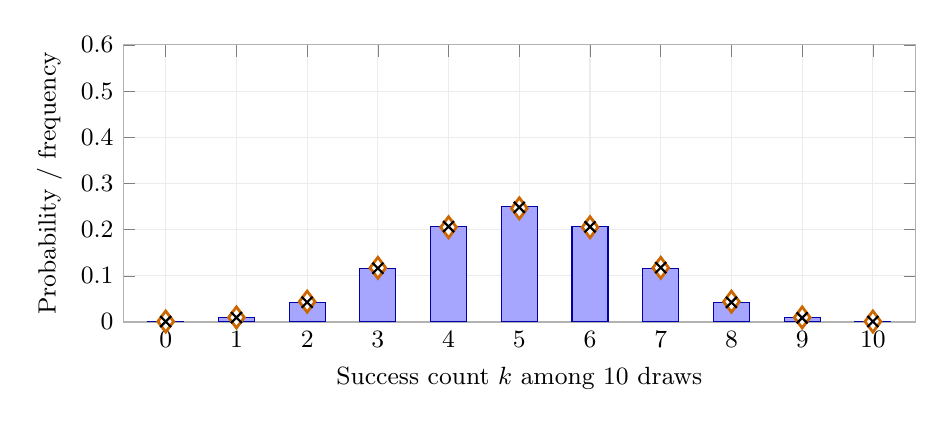
\begin{tikzpicture}
\begin{axis}[
  width=0.96\linewidth,height=5.1cm,
  xmin=-0.6,xmax=10.6,ymin=0,ymax=0.60,
  xtick={0,1,...,10},ytick={0,0.1,...,0.6},
  xlabel={Success count $k$ among $10$ draws},ylabel={Probability / frequency},
  tick label style={font=\small},label style={font=\small},
  scaled y ticks=false,grid=major,grid style={gray!15},
  axis line style={gray!60}]
\addplot[ybar,bar shift=0pt,bar width=13pt,
  fill=blue!35,draw=blue!65!black] coordinates {
  (0,0.00087025887724498)
  (1,0.009112658400471)
  (2,0.042502008320947)
  (3,0.11627492431844)
  (4,0.20662773277724)
  (5,0.24922483461131)
  (6,0.20662773277724)
  (7,0.11627492431844)
  (8,0.042502008320947)
  (9,0.009112658400471)
  (10,0.00087025887724498)
};
\addplot[only marks,mark=diamond*,mark size=3.8pt,
  color=orange!80!black,mark options={fill=white,line width=1pt}] coordinates {
  (0,0.0009765625)
  (1,0.009765625)
  (2,0.0439453125)
  (3,0.1171875)
  (4,0.205078125)
  (5,0.24609375)
  (6,0.205078125)
  (7,0.1171875)
  (8,0.0439453125)
  (9,0.009765625)
  (10,0.0009765625)
};
\addplot[only marks,mark=x,mark size=2.8pt,
  color=black,mark options={line width=0.8pt}] coordinates {
  (0,0.00085)
  (1,0.00948)
  (2,0.0427)
  (3,0.11634)
  (4,0.20655)
  (5,0.24818)
  (6,0.20599)
  (7,0.11759)
  (8,0.04252)
  (9,0.00882)
  (10,0.00098)
};
\end{axis}
\end{tikzpicture}
\end{minipage}

\par\medskip
\noindent\textbf{Measure the difference using exact probabilities.}
The common mean is $np=5$. Sampling without replacement reduces the variance:
\[
 \operatorname{Var}(X_N)=np(1-p)\frac{N-n}{N-1}
 =2.5\frac{N-10}{N-1}\longrightarrow 2.5.
\]
The total variation distance compares the two complete probability tables:
\[
 d_{\mathrm{TV}}(X_N,B)=\frac12\sum_{k=0}^{10}
 \left|\Pr(X_N=k)-\Pr(B=k)\right|,
 \qquad B\sim\operatorname{Bin}(10,1/2).
\]
It is the largest difference in probability the two models assign to the
same event. Here it is calculated from exact formulas, not simulated counts.

\begin{center}
\small
\begin{tabular}{rrrrr}
\hline
$N$ & $K$ & Sample fraction $n/N$ & Exact variance & Exact $d_{\mathrm{TV}}$\\
\hline
12 & 6 & 83.33\% & 0.454545 & 0.343750\\
40 & 20 & 25.00\% & 1.923077 & 0.070407\\
400 & 200 & 2.50\% & 2.443609 & 0.006230\\
\hline
\multicolumn{3}{l}{Binomial limit, $n=10$, $p=1/2$} & $2.500000$ & $0$\\
\hline
\end{tabular}
\end{center}

\noindent\small\textbf{How to read the comparison.}
For $N=12$, drawing $10$ of the $12$ objects forces the count into $4,5,6$.
The binomial model still assigns mass to $0,\ldots,10$, so it is a poor
approximation. As $N$ grows with $n$ fixed, the sample fraction becomes small,
the variance approaches $2.5$, and the exact bars approach the orange marks.
We are keeping $n$ fixed: this is a binomial limit, not a normal approximation.

\noindent\small\textbf{Simulation illustrates; it does not prove convergence.}
The three populations use seeds $20260942$, $20260970$, and $20261330$
(base seed $20260930$ plus $N$), with $100{,}000$ repetitions each.
The black crosses fluctuate around the exact blue bars. In the last panel,
sampling noise can obscure the small remaining difference from the binomial
model. The limit requires the mathematical PMF argument; neither a simulation
nor three finite comparisons prove it.
\endgroup
